\chapter{Ala ma kota}

ĄĆĘŁŃÓŚŹŻ ąćęłńóśźż\footnote{Przykład użycia polskich znaków diakrytycznych oraz przypisu w~miejscu}. \lipsum[1]

\section{Odniesienie do pozycji z~literatury (strona WWW)}

% Odniesienie do rysunku i~cytowanie dokumentu. Dokumenty są definiowane w~pliku literatura.bib
Reszta dokumentacji znajduje się w\cite{docker_compose_reference}. \lipsum[3]

\section{Odniesienie do książki}

Jak pisze Harel w\cite{harel_rzecz_2008}: \lipsum[7]

\section{Rysunek}

% Rysunek
\begin{figure}
    \centering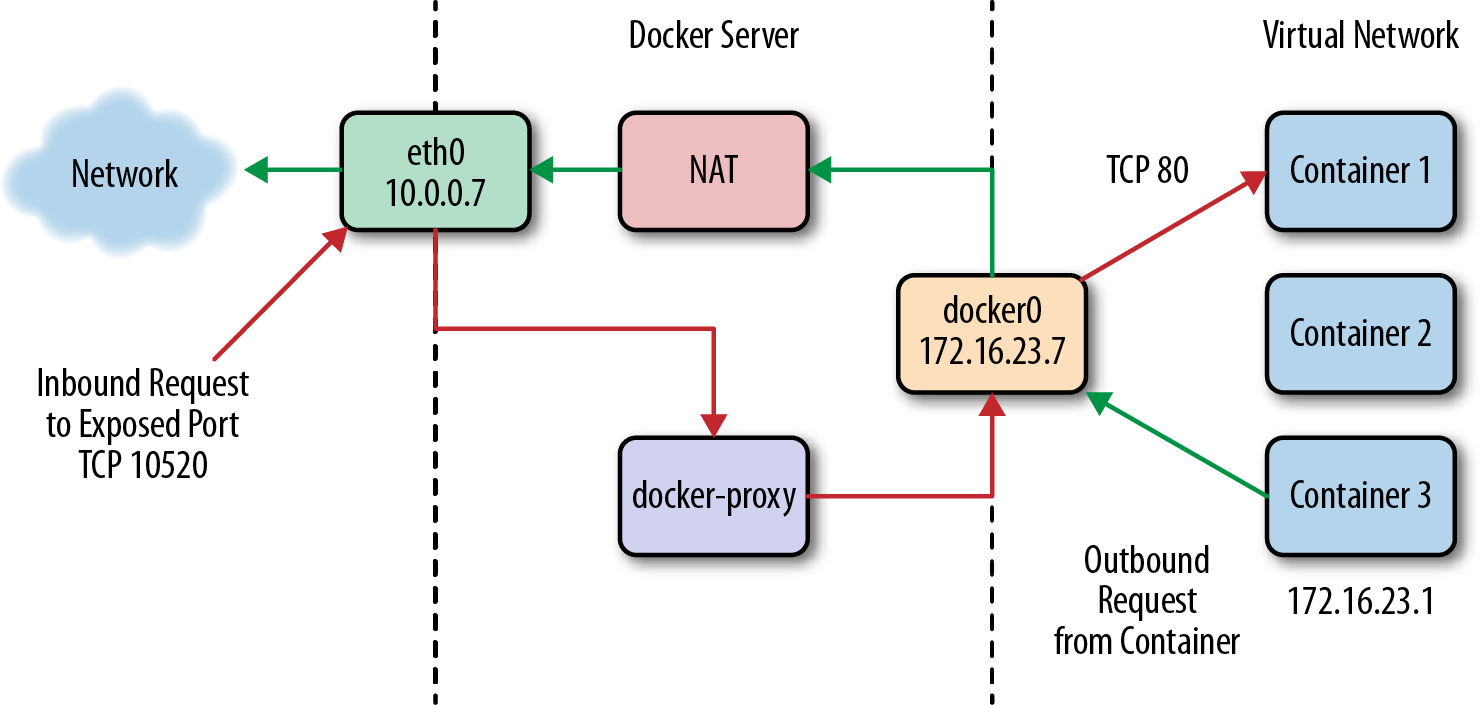
\includegraphics[width=.6\textwidth]{demo/img/swarm-network}
    \caption{Docker ma sieć\cite{docker_compose_reference}.}  \label{rys:network}
    % Źródło rysunku i~etykieta przez którą odwołujemy się do rysunku.
\end{figure}

Jak widać na rys. \ref{rys:network} Docker ma wewnętrzną sieć. \lipsum[1]


\subsection{Rysunek z~kotem}

Jak widać na rys.\ref{rysunek:kot} Ala ma kota. \lipsum[9-10]

\begin{figure}[H]
    \centering
\includegraphics[width=.4\textwidth]{demo/img/kotek}
    \caption{Ala ma kota \source{\ownwork}.}\label{rysunek:kot}
\end{figure}

\subsection{Tabela}

Co uwzględniono w~tabeli \ref{tabela:coktoma}. \lipsum[13-15]

% Tabela. Nazwa tabeli u~góry.
\begin{table}[h!]
    \centering\caption{Co kto ma\cite{harel_rzecz_2008} (patrz też dodatek~\ref{Dod1}) \label{tabela:coktoma}}
    \begin{tabular}{|l|l|l|}% wyrównanie kolumn tabeli -> l~c r~- do lewej, środka, do prawej
        \hline
        Ala & ma & kota \\
        \hline
        Ola & ma & psa \\
        \hline
        Ula & ma & małpę\\
        \hline
    \end{tabular}
\end{table}

\lipsum[19-20] Warto wspomnieć, że w\cite{aizawa_groundwater_2009} rzecz przedstawiona jest zupełnie inaczej. Poniższy wzór:

\begin{equation}
    \sum_{i=1}^{\infty}a_i
    \label{eq:mojWzor}
\end{equation}

Wzór \ref{eq:mojWzor} wskazuje że dowód podany w\cite{kaleta_experimental_2005} może zostać podważony. \lipsum[9]

\section{Kod źródłowy}

% lub {java} albo {bash} albo {text}
\begin{listing}[h!]
    \begin{minted}{c}
        int main()
        {
        int a=2*3;
        printf("**Ala ma kota\n**");
        while(!I2C_CheckEvent(I2C1, I2C_EVENT_MASTER_MODE_SELECT)); /* EV5 */
        return 0;
        }
    \end{minted}
    \caption{Przykładowy algorytm w~języku C~\source{\ownwork}} \label{listing:moj}
\end{listing}

W~moim kodzie \ref{listing:moj} zrobiłem coś wspaniałego. \lipsum[4]

\thispagestyle{normal}
